\documentclass[11pt,letterpaper]{article}

% ── Packages ──────────────────────────────────────────────
\usepackage[margin=1in]{geometry}
\usepackage{amsmath,amssymb}
\usepackage{mathtools}
\usepackage{booktabs}
\usepackage{enumitem}
\usepackage{hyperref}
\usepackage[dvipsnames]{xcolor}
\usepackage{titlesec}
\usepackage{microtype}
\usepackage{parskip}
\usepackage{tikz}
\usetikzlibrary{arrows.meta,positioning,calc,fit}

% ── Formatting ────────────────────────────────────────────
\hypersetup{colorlinks=true, linkcolor=NavyBlue, citecolor=NavyBlue, urlcolor=NavyBlue, pdfstartview=FitH}
\titleformat{\section}{\large\bfseries}{\thesection}{1em}{}
\titleformat{\subsection}{\normalsize\bfseries}{\thesubsection}{1em}{}
\titleformat{\subsubsection}{\normalsize\itshape}{\thesubsubsection}{1em}{}

% ── Math shortcuts ────────────────────────────────────────
\newcommand{\bfa}{\mathbf{a}}
\newcommand{\bfp}{\mathbf{p}}
\newcommand{\bfz}{\mathbf{z}}
\newcommand{\bfy}{\mathbf{y}}
\newcommand{\bfd}{\mathbf{d}}
\newcommand{\cS}{\mathcal{S}}
\newcommand{\R}{\mathbb{R}}
\newcommand{\pp}{\,\text{pp}}

\begin{document}

% ── Title ─────────────────────────────────────────────────
\begin{center}
{\LARGE\bfseries Neural Field Perceiver}\\[6pt]
{\large Cross-Patient Speech Decoding from Intra-Operative $\mu$ECoG\\via Spatially-Grounded Electrode Encoding}\\[12pt]
{\normalsize Ben Tang \quad\textbar\quad Greg Cogan Lab, Duke University}\\[4pt]
{\normalsize April 2026 \quad\textbar\quad Version 12}
\end{center}

\medskip\noindent\rule{\textwidth}{0.4pt}\medskip

\noindent Technical design document. \textbf{One idea}: each patient's electrode array is a partial, noisy observation of a shared neural manifold for speech production. We recover this manifold via atlas-grounded VE cross-attention at Brainnetome positions, mapping variable electrode counts into a fixed-size common space. Per-patient diagonal normalization and rigid coordinate correction calibrate each ``view.'' An autoregressive decoder generates 3-phoneme sequences via beam search over 52 valid CVC/VCV tokens. Training: external chronic ECoG SSL (JEPA with temporal masking, 50--100\,h) $\to$ per-patient supervised fine-tuning. Electrode self-attention before VE cross-attention is a first-class ablation (A\_elec\_attn).

Claims labeled \textbf{supported}, \textbf{observed}, or \textbf{hypothesis}.
Structural assumptions that could be wrong: \textcolor{BrickRed}{red}.

\tableofcontents
\newpage


%% ====================================================================
%%  SECTION 1: PROBLEM
%% ====================================================================

\section{Problem}\label{sec:problem}

Each patient's $\mu$ECoG array is a sparse spatial sample of cortical high-gamma activity (HGA, 70--150\,Hz, 200\,Hz) during speech. The array sits on left ventral sensorimotor cortex (vSMC), and electrode positions in MNI-152 space are determined post-hoc from surgical reconstruction.

\textbf{Hardware.} LCP thin-film arrays (Dyconex~\cite{duraivel2023}), physically flexible --- they conform to cortical curvature. Two configurations:

\begin{table}[ht!]\centering\small
\begin{tabular}{@{}lll@{}}
\toprule
& \textbf{128-ch (DBS)} & \textbf{256-ch (craniotomy)} \\
\midrule
Grid & $8 \times 16$ & $12 \times 22$ \\
Pitch & 1.33\,mm & 1.72\,mm \\
Footprint & ${\sim}11 \times 21$\,mm & ${\sim}21 \times 38$\,mm \\
Contact diameter & 200\,$\mu$m & 200\,$\mu$m \\
\bottomrule
\end{tabular}
\end{table}

\textbf{Task.} Non-word repetition (intra-operative, immediate --- no imposed delay): 52 CVC/VCV tokens, 9 phonemes, 3 positions per token. Output: three 9-way classifications per trial. Full-trial input (default $t_{\min}{=}{-}0.2$, $t_{\max}{=}1.0$\,s relative to response onset, pending Phase 0 sweep). Stimulus-to-response delay is $1.1 \pm 0.3$\,s~\cite{duraivel2023}, so the auditory stimulus ends ${\sim}$400\,ms before $t_{\min}$. Autoregressive decoder generates $[\text{phoneme}_1, \text{phoneme}_2, \text{phoneme}_3]$ sequentially; eliminates MFA dependency.

\textbf{Cross-patient challenge.} Arrays are offset 15--25\,mm in MNI space with variable rotation. Channel indices are meaningless across patients. Current LOPO achieves PER\,=\,0.762 (S14, grouped-by-token CV) using a per-patient Conv2d read-in that ignores electrode coordinates entirely. 55 architecture/training experiments converge to PER 0.750--0.780, suggesting a systematic barrier.

\textbf{Constraints.}

\begin{table}[ht!]\centering\small
\begin{tabular}{@{}llr@{}}
\toprule
\textbf{Constraint} & \textbf{Value} & \textbf{Impact} \\
\midrule
Sig.\ electrodes/patient & 63--201 & Sparse cortical sampling \\
Cross-patient offset & 15--25\,mm & Different cortex sampled \\
Trials/patient & 46--178 & Small-data regime \\
Utterance/patient & ${\sim}$1\,min & SSL has failed \\
Patients & ${\sim}$10 & Too few for large models \\
\bottomrule
\end{tabular}
\end{table}

\textbf{Why coordinates might help.} Per-patient Conv2d learns spatial filters independently --- nothing is spatially shared. If two patients sample the same cortical region, the model cannot exploit this. MNI coordinates make spatial correspondence explicit.


%% ====================================================================
%%  SECTION 2: IDEA
%% ====================================================================

\section{Idea: Spatially-Grounded Electrode Encoding}\label{sec:idea}

\subsection{What we assume}

Speech motor cortex has \textbf{conserved somatotopic organization}: gross ordering (medial$\to$lateral: leg$\to$hand$\to$face) is invariant~\cite{roux2020}; functional connectivity is the most conserved feature~\cite{mueller2013}. Fine structure varies by ${\sim}$15--25\,mm~\cite{eichert2020}. The spatial map exists; its absolute position varies.

\textcolor{BrickRed}{\textit{Untested:}} That this conservation is strong enough, at $\mu$ECoG resolution, to transfer across $N{=}10$ patients with centimeter-scale positional uncertainty.

\subsection{The core components}\label{sec:components}

The idea has three components, motivated by multi-view reconstruction:

\begin{enumerate}[leftmargin=2em]
\item \textbf{Per-patient calibration.} Diagonal normalization ($s^{(i)} \odot x + b^{(i)}$) absorbs impedance/gain. Learned rigid correction ($\Delta^{(i)}, \omega^{(i)}$) absorbs registration error. Per-patient VE position offsets ($\delta_l^{(i)}$, leashed $\leq$15\,mm) adapt atlas positions to individual somatotopy. These are the ``camera intrinsics and extrinsics.''

\item \textbf{Atlas-grounded virtual electrodes.} $L{=}16$ query vectors at per-patient-adapted Brainnetome positions (atlas centroid + learned offset) cross-attend to real electrodes with a distance bias, mapping variable-count electrodes into a \textbf{common functional space} --- the ``template mesh.'' The atlas ($N{=}40$ HCP subjects~\cite{fan2016}) provides the spatial prior; per-patient offsets (48\,params) adapt to individual variation.

\item \textbf{Temporal self-attention.} Self-attention among VE tokens across time captures articulatory dynamics. Temporal span masking during SSL (Section~\ref{sec:ssl}) teaches the model to predict missing temporal content from context.
\end{enumerate}

Total per-patient params: ${\sim}$182 (128 diagonal + 6 geometric + 48 VE offsets). Far below BIT (6M/pt), Willett (65.8K/day), seegnificant (2K/subject). Details in Sections~\ref{sec:tokens}--\ref{sec:ve-crossattn}.


%% ====================================================================
%%  SECTION 3: ARCHITECTURE
%% ====================================================================

\section{Architecture}\label{sec:architecture}

\begin{center}
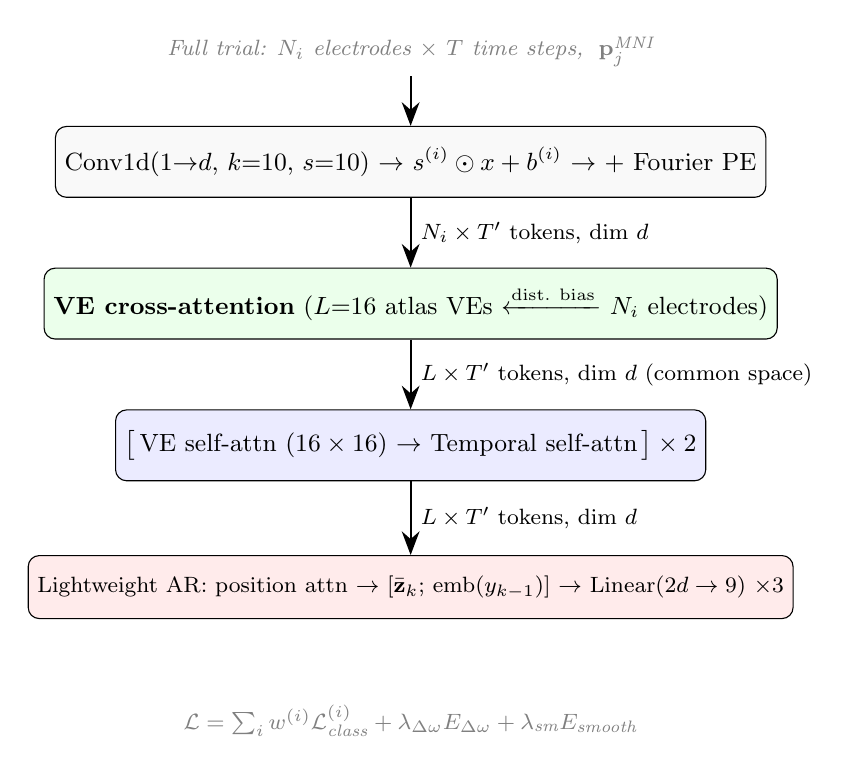
\begin{tikzpicture}[
  box/.style={draw, rounded corners, minimum width=6cm, minimum height=0.9cm, align=center, font=\small},
  smallbox/.style={draw, rounded corners, minimum width=6cm, minimum height=0.8cm, align=center, font=\footnotesize},
  arrow/.style={-{Stealth[length=3mm]}, thick},
  label/.style={font=\footnotesize\itshape, text=gray}
]

\node[box, fill=gray!5] (input) at (0, 2.7) {Conv1d($1{\to}d$, $k{=}10$, $s{=}10$) $\to$ $s^{(i)} \odot x + b^{(i)}$ $\to$ + Fourier PE};

\node[box, fill=green!8] (ve) at (0, 0.9) {\textbf{VE cross-attention} ($L{=}16$ atlas VEs $\xleftarrow{\text{dist. bias}}$ $N_i$ electrodes)};

\node[box, fill=blue!8] (block) at (0, -0.9) {$\bigl[$\,VE self-attn ($16 \times 16$) $\to$ Temporal self-attn\,$\bigr] \times 2$};

\node[smallbox, fill=red!8] (decoder) at (0, -2.7) {Lightweight AR: position attn $\to$ $[\bar{\bfz}_k;\, \text{emb}(y_{k-1})]$ $\to$ Linear($2d \to 9$) $\times 3$};

\node[label] (raw) at (0, 4.1) {Full trial: $N_i$ electrodes $\times$ $T$ time steps, $\;\bfp_j^{\text{MNI}}$};

\draw[arrow] (raw) -- (input);
\draw[arrow] (input) -- (ve) node[midway, right, font=\footnotesize] {$N_i \times T'$ tokens, dim $d$};
\draw[arrow] (ve) -- (block) node[midway, right, font=\footnotesize] {$L \times T'$ tokens, dim $d$ (common space)};
\draw[arrow] (block) -- (decoder) node[midway, right, font=\footnotesize] {$L \times T'$ tokens, dim $d$};

\node[label] at (0, -4.4) {$\mathcal{L} = \sum_i w^{(i)} \mathcal{L}^{(i)}_{\text{class}} + \lambda_{\Delta\omega} E_{\Delta\omega} + \lambda_{\text{sm}} E_{\text{smooth}}$};

\end{tikzpicture}
\end{center}

\begin{equation}
\boxed{\mathcal{L}_{\text{supervised}} = \sum_i w^{(i)} \frac{1}{3}\sum_{k=1}^{3} \text{FocalCE}(\hat{y}_k, y_k) + \lambda_{\Delta\omega} E_{\Delta\omega} + \lambda_{\text{sm}} E_{\text{smooth}}}
\end{equation}
\begin{equation}
\boxed{\mathcal{L}_{\text{SSL}} = \text{JEPA}_{L_1} \text{ with temporal masking, content-aware weighting, } r \sim \text{U}(0,1) \quad \text{(Section~\ref{sec:ssl-objective})}}
\end{equation}


\subsection{Electrode tokens}\label{sec:tokens}

Each electrode is a point in MNI space with a scalar HGA time series. Tokenization:

\begin{equation}
\text{token}_j(t') = \underbrace{s^{(i)} \odot \text{Conv1d}(x_j;\; k{=}10,\, s{=}10)_{t'} + b^{(i)}}_{\text{per-patient normalized activity}} + \underbrace{\text{Linear}\bigl(\gamma(\tilde{\bfp}_j)\bigr)}_{\text{position (constant)}} + \underbrace{\text{sinPE}(t')}_{\text{temporal index}}
\end{equation}

\textbf{Temporal binning (shared).} Conv1d($1 \to d$, $k{=}10$, $s{=}10$): maps each electrode's scalar HGA to $d$-dim tokens at non-overlapping 50\,ms windows (200\,Hz $\to$ $T'$ time bins). Default: $t_{\min}{=}{-}0.2$, $t_{\max}{=}1.0$ ($T'{=}24$), pending Phase 0 sweep. Shared across all electrodes and patients.

\textbf{Per-patient diagonal normalization.} $s^{(i)} \odot x + b^{(i)}$, $s^{(i)}, b^{(i)} \in \R^d$ (128 params/patient). \textbf{Initialized from channel statistics}~\cite{karpowicz2025nomad}: $s^{(i)}_k = 1/\sigma_k^{(i)}$, $b^{(i)}_k = -\mu_k^{(i)}/\sigma_k^{(i)}$. This starts as z-scoring; the model learns only the residual correction.

\textbf{Coordinate pipeline (ACPC $\to$ MNI).} Electrode coordinates are stored in ACPC space (per-patient, AC-PC aligned). Before use, they are transformed to MNI-152 via the patient's \texttt{talairach.xfm} affine, then corrected by the learned per-patient rigid calibration:
\begin{equation}
\tilde{\bfp}_j = R(\omega^{(i)}) \bigl(T^{(i)}_{\text{xfm}}\, \bfp_j^{\text{ACPC}}\bigr) + \Delta^{(i)}
\end{equation}
where $T^{(i)}_{\text{xfm}}$ is the fixed talairach transform (12-param affine, not learned) and $\Delta^{(i)}, \omega^{(i)}$ absorb residual registration error (6 learnable params/patient, hard-clamped $\|\Delta\| \leq 15$\,mm, $\|\omega\| \leq 0.15$\,rad, L2-regularized, init at $\mathbf{0}$).

\textbf{Electrode localization.} CT-MRI coregistration $\to$ grid interpolation $\to$ cortical surface projection. Error is primarily \textbf{systematic} (rigid-body ${\sim}$4--8\,mm), not random per-electrode (${\sim}$0.1\,mm) --- hence $\Delta/\omega$ rigid correction. Residual \textit{anatomical} variation (${\sim}$15--25\,mm~\cite{eichert2020}) is nonlinear and handled by VE cross-attention receptive fields (Section~\ref{sec:ve-crossattn}).

\textbf{Fourier PE ($F{=}3$).} MNI coordinates $\tilde{\bfp}_j$ (after talairach transform + learned calibration), standardized so speech motor region spans $[-1, 1]$:
\begin{equation}
\gamma(\bar{\bfp}) = \bigl[\sin(2^0 \pi \bar{\bfp}),\; \cos(2^0 \pi \bar{\bfp}),\; \ldots,\; \sin(2^{F-1} \pi \bar{\bfp}),\; \cos(2^{F-1} \pi \bar{\bfp})\bigr] \in \R^{6F}
\end{equation}
At $F{=}3$: wavelengths 30\,mm (full-array), 15\,mm (articulatory region), 7.5\,mm (sub-region). Projected via Linear($18 \to d$). Fourier PE provides \textbf{directional} identity (anisotropic), complementing the distance bias (\textbf{proximity}, isotropic). Two equidistant electrodes in different directions are indistinguishable by distance bias alone. \textbf{A3} removes PE; \textbf{A11} sweeps $F$.


\subsection{Electrode self-attention (ablation A\_elec\_attn)}\label{sec:elec-selfattn}

\textbf{Not in the default pipeline.} The default sends electrode tokens directly to VE cross-attention. Electrode self-attention is an ablation testing whether local spatial preprocessing helps.

\textbf{Why not default.} Electrode self-attention learns spatial relationships \textit{within} each patient's array. The shared Q/K/V weights operate on tokens containing Fourier PE of MNI coordinates. But the functional meaning of any given MNI location varies substantially across patients (spatial gradient $R^2 = 0.05$--$0.13$; Duraivel 2025). Content-based attention patterns tied to absolute coordinates are patient-specific and unlikely to transfer. The only transferable component is distance-based smoothing (nearby electrodes correlate --- physics, not neuroscience), which does not require learned Q/K/V.

\textbf{A\_elec\_attn} inserts one layer of distance-biased self-attention before VE cross-attention:
\begin{equation}
A_{jk} = \frac{Q_j \cdot K_k}{\sqrt{d_h}} - \alpha_h^{\text{elec}} \|\tilde{\bfp}_j - \tilde{\bfp}_k\|^2
\end{equation}
${\sim}$16K params (4 heads, $d{=}64$), $O(N_i^2)$ per patient per time bin. If A\_elec\_attn $>$ default, local spatial gradients carry information lost by VE point-sampling; it becomes the new default. \textbf{A\_elec\_attn\_no\_pe} tests the same layer but with distance bias only (no Fourier PE on electrode tokens), isolating generic spatial smoothing from position-specific patterns.


\subsection{VE cross-attention (spatial aggregation)}\label{sec:ve-crossattn}

$L{=}16$ virtual electrode queries cross-attend to the patient's $N_i$ electrode tokens, producing a fixed-size $L \times d$ representation per time bin. VE positions are \textbf{per-patient}: atlas centroid + learned offset, leashed to prevent drift:
\begin{equation}
\bfp_l^{(i)} = \bfp_l^{\text{atlas}} + \delta_l^{(i)}, \quad \|\delta_l^{(i)}\| \leq 15\,\text{mm}, \quad \delta_l^{(i)} \text{ init } \mathbf{0}
\end{equation}
48 params/patient ($L{=}16 \times 3$ coordinates), L2-regularized. The atlas provides a strong spatial prior ($N{=}40$ HCP subjects); the offset adapts to each patient's individual somatotopy (varies by 5--15\,mm). Cross-attention:
\begin{equation}
A_{lj} = \frac{Q_l \cdot K_j}{\sqrt{d_h}} - \alpha_h \|\bfp_l^{(i)} - \tilde{\bfp}_j\|^2
\end{equation}
The distance bias determines \textit{where} to look (per-patient, via leashed positions). The Q/K/V determines \textit{what} to extract (shared --- VE query learns ``I am tongue M1, extract tongue-related temporal features'' regardless of which patient). This separation is key: spatial selection is per-patient, functional selectivity is shared. At $\alpha_h \approx 0.003$: ${\sim}$25\,mm soft receptive fields.

\textbf{A\_no\_deform:} Fix VE positions at atlas centroids (no per-patient offsets). Tests whether individual somatotopic adaptation matters.

\textbf{A\_dist\_only:} Remove Q/K/V from cross-attention entirely (distance-only pooling: $w_{lj} = \text{softmax}(-\alpha \|\bfp_l^{(i)} - \tilde{\bfp}_j\|^2)$, $z_l = \sum_j w_{lj} x_j$). Tests whether functional selectivity matters beyond spatial proximity.

\textbf{Per-electrode uncertainty weighting}~\cite{hewitt2024}. Each electrode predicts $\sigma_j > 0$ (Linear($d \to 1$) + softplus, ${\sim}$65 params), modulating cross-attention:
\begin{equation}
A_{lj} = \frac{Q_l \cdot K_j}{\sqrt{d_h}} - \alpha_h \|\bfp_l^{(i)} - \tilde{\bfp}_j\|^2 - \beta_h \log \sigma_j^2
\end{equation}

\textbf{VE content vectors.} Learned $c_l \in \R^d$ per VE (shared). Queries: $Q_l = W_Q(c_l + \text{FourierPE}(\bfp_l^{(i)}))$. Fourier PE uses the per-patient VE position, so query embeddings adapt to each patient's atlas deformation. Initialized from functional profiles: mean HGA response per ROI across reachable patients, projected to $d$-dim via PCA.


\subsection{Spatiotemporal blocks ($\times B$)}\label{sec:blocks}

After VE cross-attention, the representation is $L \times T'$ tokens ($L{=}16$ VEs $\times$ 24 time bins). Each block alternates:

\textbf{(a) VE spatial self-attention} (per time bin). The 16 VE tokens attend to each other:
\begin{equation}
A_{lm} = \frac{Q_l \cdot K_m}{\sqrt{d_h}}
\end{equation}
Standard scaled dot-product, 4 heads. Captures inter-regional communication. At $L{=}16$: $256$ entries per time bin.

\textbf{(b) Temporal self-attention} (per VE). Each VE attends across 24 time bins. 4 heads, sinusoidal temporal PE.

\textbf{Factored vs.\ combined attention.} Default factors spatial and temporal. seegnificant~\cite{mentzelopoulos2024}: factored $>$ joint at electrode-level ($+0.06\; R^2$). BarISTA~\cite{oganesian2025}: combined $>$ factored by 1--2\pp{} at parcel-level, closer to our $L{=}16$ VEs. At $16 \times 24 = 384$ tokens, cost is trivial either way. \textbf{A\_combined} tests joint spatiotemporal self-attention.

\textbf{Block internals.} Pre-LN residual connections, ReLU FFN ($d_\text{ff} = 4d$), dropout $p{=}0.2$, DropPath $p{=}0.1$. Channel dropout ($p{=}0.2$) applied to electrode tokens \textit{before} VE cross-attention as input regularization.


\subsection{Virtual electrode atlas positions ($L{=}16$)}\label{sec:ve-atlas}

16 left-hemisphere Brainnetome ROI centroids~\cite{fan2016}, selected as the top 16 by patient reachability ($<$25\,mm) from all 123 LH ROIs. All have ${\geq}3$ patients within 25\,mm. Brainnetome over HCP-MMP1.0~\cite{glasser2016} because Brainnetome provides somatotopic motor/sensory subdivisions (tongue M1, face M1, tongue S1) --- HCP-MMP's area 4 centroid is at the dorsal hand region, ${\sim}$30\,mm from the ventral face/tongue cortex our arrays cover.

\begin{itemize}[leftmargin=2em]
\item \textbf{Motor} (3): A6cvl (ventral PMC, 9\,pts), A4tl (tongue M1, 7\,pts), A4hf (face M1, 6\,pts)
\item \textbf{Sensory} (3): A1/2/3tonIa (tongue S1, 8\,pts), A1/2/3ulhf (face S1, 5\,pts), A2 (proprioceptive S1, 3\,pts)
\item \textbf{Broca's} (6): A44d (8\,pts), A45c (8\,pts), A44v (7\,pts), A45i (7\,pts), A45r (5\,pts), A44op (opercular, 4\,pts)
\item \textbf{Auditory} (2): STGpp (planum polare, 4\,pts), STGa (anterior STG, 4\,pts)
\item \textbf{Insula} (1): INSa (articulatory planning, 4\,pts)
\item \textbf{Executive} (1): MFG (dorsolateral PFC, 6\,pts)
\end{itemize}

Broca's-heavy (6/16) because the anterior-ventral electrode cluster (S26, S32, S33, S57) covers IFG well. SMA/pre-SMA unreachable (0 patients, too medial).

\textbf{Patient-adaptive masking.} \texttt{select\_active\_virtual\_electrodes()} masks VEs with no electrode within 25\,mm. Each patient reaches ${\sim}$6--12 of 16 VEs. Masked VEs receive zero attention weight, not learned content.


\subsection{Learned spatial alternative (ablation)}\label{sec:learned-spatial}

\textbf{A\_self\_attn: Electrode self-attention (no atlas).} Replace VE cross-attention with self-attention among $N_i$ electrodes per time bin + Fourier PE. Decoder cross-attends to $N_i \times T'$ tokens (variable size). Follows seegnificant~\cite{mentzelopoulos2024}.

\textbf{E2.1: Learned latents (no atlas).} Replace atlas positions with $L{=}16$ learned position vectors. Same Perceiver cross-attention, same bottleneck, everything else identical. Isolates atlas from bottleneck. If learned latents match atlas at $N{=}10$, the atlas is a convenience. If atlas wins at small $N$, that's the core finding.


\subsection{Phoneme decoder}\label{sec:phoneme-decoder}

\textbf{Default: lightweight autoregressive heads.} Three position-specific heads with AR conditioning --- each step sees the previous phoneme:

\begin{enumerate}[leftmargin=2em]
\item \textbf{Temporal pooling per position.} Learned position embeddings $q_k \in \R^d$ ($k{=}1,2,3$) attend to the $T'{=}24$ time bins via cross-attention (single head): $\text{attn}_k = \text{softmax}(q_k \cdot K / \sqrt{d})$, producing $\bar{\bfz}_k \in \R^{L \times d}$. Position 1 attends to premotor/onset, position 3 to offset.
\item \textbf{Spatial pooling.} Mean-pool over $L{=}16$ VEs: $\bar{\bfz}_k \in \R^d$.
\item \textbf{AR conditioning.} Concatenate with previous phoneme embedding: $[\bar{\bfz}_k;\; \text{emb}(y_{k-1})] \in \R^{2d}$. Step 1 receives a learned BOS token. During training: teacher forcing (ground-truth $y_{k-1}$). During inference: predicted $\hat{y}_{k-1}$.
\item \textbf{Classification.} Linear($2d \to 9$) $\to$ 9-way softmax per position.
\end{enumerate}

${\sim}$4.1K params total ($16\times$ lighter than a full transformer decoder).

\textbf{Training:}
\begin{equation}
\mathcal{L}_\text{class} = \frac{1}{3}\sum_{k=1}^{3} \text{FocalCE}(\hat{y}_k, y_k;\; \gamma{=}2,\; \text{LS}{=}0.1) \quad \text{with mixup } (\alpha{=}0.2)
\end{equation}

\textbf{Inference: beam search with 52-token constraint.} Beam search ($B{=}8$) over the 3-step AR sequence, constrained to 52 valid CVC/VCV tokens ($52/729 = 7.1\%$ of output space).

\textbf{A\_no\_ar}: remove AR conditioning entirely (independent position heads, no previous phoneme embedding). Tests whether inter-phoneme modeling is worth ${\sim}$2K params.


\subsection{Parameter budget}

\begin{table}[ht!]\centering\small
\begin{tabular}{@{}lrll@{}}
\toprule
\textbf{Module} & \textbf{Params} & \textbf{Shared?} & \textbf{Note} \\
\midrule
Conv1d($1 \to d$, $k{=}10$) & ${\sim}$0.7K & Shared & Temporal binning \\
Fourier PE + Linear (electrodes) & ${\sim}$1.2K & Shared & Directional spatial identity \\
VE content + Fourier PE & ${\sim}$2.2K & Shared & $L{=}16$ learned content + position \\
VE cross-attention & ${\sim}$33K & Shared & $Q, K, V, O$ projections + dist.\ bias \\
Blocks ($\times B$) & ${\sim}$66$B$K & Shared & VE self-attn ($16 \times 16$) + temporal self-attn + FFN \\
Lightweight AR decoder & ${\sim}$4.1K & Shared & Phoneme emb + $3 \times$ (pos attn + Linear($2d \to 9$)) \\
\midrule
$s^{(i)}, b^{(i)}$ (diagonal) & 128/pt & Per-patient & Signal normalization \\
$\Delta^{(i)} + \omega^{(i)}$ & 6/pt & Per-patient & Registration correction \\
$\delta_l^{(i)}$ (VE offsets) & 48/pt & Per-patient & Per-patient VE positions ($16 \times 3$) \\
\midrule
JEPA target enc.\ (EMA) + predictor (SSL only) & ${\sim}$16K & Shared & Predictor: Linear($d{\to}2d$) + GELU + Linear($2d{\to}d$); target: EMA of encoder \\
AR decoder (A\_ar only) & ${\sim}$67K & Shared & 1-layer transformer + embeddings (ablation) \\
\midrule
\textbf{Shared ($B{=}2$, supervised)} & $\mathbf{{\sim}173}$\textbf{K} & & VE cross-attn 33K + 2 blocks 132K + decoder 4K + PE/embed 4K \\
\textbf{Shared ($B{=}2$, SSL)} & $\mathbf{{\sim}189}$\textbf{K} & & $+$ JEPA predictor 16K (discarded after SSL) \\
\textbf{Shared ($B{=}1$, supervised)} & $\mathbf{{\sim}107}$\textbf{K} & & Ablation A10 \\
\textbf{Per-patient ($\times$10)} & $\mathbf{{\sim}1.8}$\textbf{K} & & 182/pt --- deliberately lean \\
\textbf{Total ($B{=}2$)} & $\mathbf{{\sim}175}$\textbf{K} & & Encoder-heavy: 96\% in spatial/temporal processing \\
\bottomrule
\end{tabular}
\end{table}

\textcolor{BrickRed}{\textit{Capacity:}} ${\sim}$175K total ($B{=}2$), 182/pt (including 48 VE offsets). Fine-tuning on ${\sim}$1{,}300 trials safe via gradual unfreezing (steps 1--2 train ${\sim}$5K params). \textbf{A10} tests $B \in \{1, 2, 3\}$.


%% ====================================================================
%%  SECTION 4: TRAINING
%% ====================================================================

\section{Training and Evaluation}\label{sec:training}

\subsection{Phase 1: Source training}

$N{-}1$ source patients. AdamW ($10^{-3}$), geometric params ($\Delta, \omega$) at $3 \times 10^{-4}$. Cosine decay with 20-epoch warmup. Weight decay $10^{-4}$, grad clip 5.0, batch 16. Early stopping on 20\% held-out source validation, patience 7.

\subsection{Phase 2: Target adaptation}

Per fold of 5-fold grouped-by-token CV on target patient:

\textbf{Option A: Gradual unfreezing (default).} Following the POYO/POSSM/FALCON consensus~\cite{ryoo2025possm,karpowicz2024falcon}, progressively unfreeze layers instead of binary LP$\to$FT. Each step trains until validation loss plateaus (patience 7), then unfreezes the next layer group:
\begin{enumerate}[leftmargin=2em]
\item \textbf{Per-patient calibration.} Freeze all shared weights. Train per-patient params ($s^{(\text{tgt})}, b^{(\text{tgt})}, \Delta^{(\text{tgt})}, \omega^{(\text{tgt})}, \delta_l^{(\text{tgt})}$) only. Target data only. Init $s^{(\text{tgt})}$ from $1/\sigma(\text{channels})$, $b^{(\text{tgt})}$ from $-\mu/\sigma$ (channel statistics; see Section~\ref{sec:tokens}); $\delta_l$ init at $\mathbf{0}$ (atlas centroid).
\item \textbf{$+$ AR decoder.} Unfreeze decoder (phoneme embeddings, position embeddings, cross-attention, output projection). Target data only.
\item \textbf{$+$ Last spatiotemporal block.} Unfreeze the final block at $0.1\times$ LR. \textbf{Source replay}: 70\% target + 30\% source data (uniform across source patients)~\cite{levin2026}. Prevents catastrophic forgetting of shared representations.
\item \textbf{$+$ All shared weights.} Unfreeze remaining shared weights at $0.1\times$ LR. Same 70/30 replay. Patience 5 (shorter --- diminishing returns from full fine-tuning with limited data).
\end{enumerate}
\textbf{Option B: Test-time optimization (ablation A\_tto).} Freeze encoder+decoder. Optimize only per-patient params (182 variables: 128 diagonal + 6 geometric + 48 VE offsets) via L-BFGS on ${\sim}$20--50 calibration trials~\cite{hewitt2024}. If the backbone is sufficiently good, TTO converges in seconds and approaches LP-FT --- the clinical deployment story.

\subsection{Regularization}\label{sec:regularizers}

\textbf{Default loss:}
\begin{equation}
\mathcal{L} = \sum_i w^{(i)} \mathcal{L}^{(i)}_{\text{class}} + \lambda_{\Delta\omega} E_{\Delta\omega} + \lambda_{\text{sm}} E_{\text{smooth}}
\end{equation}
where $w^{(i)}$ weights each patient by signal quality (sig channel ratio, artifact count; fixed, not learned). Two regularizers active by default:

\begin{itemize}[leftmargin=2em]
\item $E_{\Delta\omega}$: L2 on geometric params $\Delta^{(i)}, \omega^{(i)}$ ($\lambda{=}10^{-3}$). Prevents drift to the 15\,mm clamp.
\item $E_{\text{smooth}}$: Temporal smoothness $\sum_{l,t'} \|\bfz_{l,t'+1} - \bfz_{l,t'}\|^2$ (small $\lambda$). Neural activity is smooth; prevents learning high-frequency noise.
\end{itemize}

Plus standard implicit regularization: AdamW weight decay ($10^{-4}$), dropout ($p{=}0.2$), DropPath ($p{=}0.1$), channel dropout ($p{=}0.2$).

\textbf{Optional alignment losses (Phase 7).} Cross-patient contrastive (same phoneme $\to$ similar VE reps across patients) and KL distribution matching on VEs~\cite{karpowicz2025nomad}. Not default --- the architecture should produce aligned VE representations without explicit alignment pressure. Test only if Phase 4 residual analysis shows patient identity dominating the shared space.


\subsection{Evaluation}

\textbf{Zero-shot:} Phase 1 only, $\Delta{=}\omega{=}\mathbf{0}$. Pure coordinate generalization.

\textbf{LP-FT (primary):} Phase 1 $\to$ Phase 2. Matches clinical calibration.

\textbf{Metrics:} PER (edit distance on 3-phoneme sequences), grouped-by-token 5-fold CV, 3 seeds. Full recipe: weighted $k$-NN ($k{=}10$), TTA 16, beam search ($B{=}8$) with 52-token constraint.

\subsection{Diagnostics}\label{sec:diagnostics}

\begin{itemize}[leftmargin=2em]
\item \textbf{Forward prediction $R^2$:} If it stalls as patients are added, heterogeneity is the bottleneck --- switch to patient ranking~\cite{jiang2025}.
\item \textbf{Patient curriculum:} (1) Core 4, (2) $+$S39, S58, (3) $+$S23, S16, S22. Stop if validation degrades~\cite{wu2025mibrain,jiang2025}.
\item \textbf{VE reachability compatibility:} $\text{compat}(i, j) = |\text{activeVEs}(i) \cap \text{activeVEs}(j)| / |\text{activeVEs}(i) \cup \text{activeVEs}(j)|$. Rank source patients for N-curve ordering and SSL selection.
\end{itemize}

Residual analysis, VE interpretability, variance decomposition: Section~\ref{sec:phase4}.


%% ====================================================================
%%  SECTION 4.5: SSL PRETRAINING
%% ====================================================================

\section{Self-Supervised Pretraining}\label{sec:ssl}

Addresses the data bottleneck: ${\sim}$1{,}300 labeled trials vs.\ 456\,min raw continuous EDF (29 patients). Design informed by V-JEPA~2/2.1~\cite{bardes2025vjepa2,bardes2026vjepa21}, BIT~\cite{zhang2026bit}, BarISTA~\cite{oganesian2025}, BrainBERT~\cite{wang2023brainbert}, and RPNT~\cite{fang2026}.

\subsection{SSL objective: JEPA with temporal masking}\label{sec:ssl-objective}

\textbf{Design rationale.} One objective, not three. V-JEPA~2/2.1~\cite{bardes2025vjepa2,bardes2026vjepa21} --- Meta's SOTA video SSL --- uses a single JEPA loss and achieves state-of-the-art on both understanding and prediction tasks. The video SSL field's trajectory (pretext tasks $\to$ contrastive $\to$ MAE $\to$ JEPA) shows that intensifying one objective beats diversifying across many. Multi-headed losses (temporal discrimination + swap detection + JEPA) create hyperparameter coupling ($\lambda_{\text{recon}}$, swap rate, $\tau$, $\alpha$) that cannot be reliably tuned at our data scale (${\sim}$24--100\,h). Prior reasoning was: PopT~\cite{chau2025} showed discriminative $>$ reconstructive for cross-patient sEEG. But PopT's task is binary detection --- much easier than phoneme sequence decoding, where richer temporal representations are needed. JEPA learns these by construction: predicting masked temporal content forces the backbone to model articulatory dynamics. L1 loss (V-JEPA~2 recipe) over L2 for robustness to outliers. Content-aware weighting~\cite{wang2023brainbert} addresses the 68\% near-zero problem in z-scored HGA.

\subsubsection{JEPA objective}

Predict latent representations of masked VE-time positions from visible context via an EMA target encoder ($\tau{=}0.996 \to 1.0$). Content-aware weighting ($w_{t'} = 1 + \alpha \|\bar{x}_{t'}\|$, $\alpha{\approx}2$~\cite{wang2023brainbert}) upweights high-activation bins.

\begin{equation}
\mathcal{L}_{\text{SSL}} = \frac{1}{|\mathcal{M}|} \sum_{t' \in \mathcal{M}} w_{t'} \cdot \|\bfz^{\text{tgt}}_{t'} - f_{\text{pred}}(\bfz^{\text{online}}_{t'})\|_1
\end{equation}

\textbf{Masking.} Temporal span masking (max 6 patches / 300\,ms). Mask ratio $r \sim \text{U}(0, 1)$ per sample~\cite{fang2026} --- strictly better than any fixed ratio. Optional VE-level spatial masking (mask entire VE positions for some timepoints, forcing cross-VE prediction).

\textbf{Why JEPA over raw MSE:} Latent targets (EMA encoder) provide smoother learning signal than pixel-space reconstruction. BarISTA~\cite{oganesian2025} confirmed for iEEG. BrainBERT~\cite{wang2023brainbert} showed content-aware weighting is critical for sparse neural signals.

\textbf{Why not multi-headed SSL:} Electrode-level swap detection (prior design) is architecturally misaligned --- it trains representations at electrode level before VE cross-attention, but the default architecture has no electrode self-attention. The gradient doesn't reach VE or temporal layers. Temporal discrimination is a pretext task analogous to ``predict frame order'' in video --- V-JEPA showed these are superseded by masked prediction. Both are tested as ablations (A\_disc, A\_swap).

\subsubsection{Dense prediction loss (ablation A\_dense)}

Inspired by V-JEPA~2.1~\cite{bardes2026vjepa21}: supervise \textit{visible} (unmasked) tokens in addition to masked tokens, with distance-weighted supervision near mask boundaries:
\begin{equation}
\mathcal{L}_{\text{dense}} = \mathcal{L}_{\text{SSL}} + \frac{1}{|C|} \sum_{i \in C} \frac{\lambda}{\sqrt{d_{\min}(i, \mathcal{M})}} \cdot \|\bfz^{\text{tgt}}_i - f_{\text{pred}}(\bfz^{\text{online}}_i)\|_1
\end{equation}
This prevents context tokens from degenerating into global aggregators. \textbf{Caution:} V-JEPA~2.1 found context loss harms classification ($-10\pp$) unless paired with deep supervision across intermediate encoder layers. With only $B{=}2$ blocks, recovery may be limited. Not default --- test as ablation.

\textbf{If audio annotations are available} from external data: add neural-audio contrastive (CLIP-style InfoNCE~\cite{antoniades2024}) as auxiliary. One-sentence future direction, not default.

\textbf{Validation.} Downstream linear probe accuracy on a small held-out labeled set for checkpoint selection, not reconstruction $R^2$.

\subsection{Per-patient layers during SSL}

Following BIT~\cite{zhang2026bit}, per-patient diagonal normalization is learned during SSL; the backbone, target encoder, and predictor are shared.

\begin{table}[ht!]\centering\small
\begin{tabular}{@{}lll@{}}
\toprule
\textbf{Component} & \textbf{During SSL} & \textbf{During supervised} \\
\midrule
Shared Conv1d + per-patient $s^{(i)}, b^{(i)}$ & Same as supervised & Same \\
Fourier PE + Linear & Shared & Same \\
VE cross-attn + spatiotemporal blocks & Shared (encoder) & Same \\
JEPA target encoder (EMA) + predictor & Shared (${\sim}$16K) & Removed \\
Autoregressive decoder & Not used & Shared (init from scratch) \\
$\Delta^{(i)}, \omega^{(i)}$ & Learned during SSL & Transferred or reset \\
\bottomrule
\end{tabular}
\end{table}

\subsection{Data augmentation}\label{sec:augmentation}

\textbf{Signal-domain} (BIT recipe~\cite{zhang2026bit} for SSL; lighter for supervised): white noise SD\,=\,0.10--0.20, constant offset SD\,=\,0.05--0.10, amplitude scaling SD\,=\,0.15--0.25, Gaussian smoothing ($w{=}2.0$), channel dropout $p{=}0.1$. No time shift for continuous SSL data (random windowing is implicit).

\textbf{Coordinate-domain}~\cite{hewitt2024}: coordinate jitter ($\sigma{=}$2--5\,mm), global rigid perturbation ($\Delta \leq 5$\,mm), electrode subset sampling (70--100\%), VE atlas position jitter ($\sigma{=}$3--8\,mm). Teaches robust receptive fields against registration error and anatomical variation.


\subsection{SSL training recipe}

\textbf{Primary pipeline (2-stage, contingent on external data access).}
\begin{enumerate}[leftmargin=2em]
\item \textbf{Stage 1: External chronic ECoG SSL (JEPA).} Large-scale pretraining on chronic epilepsy-monitoring ECoG during speech production. Target sources: Flinker/Chen lab, NYU (48 patients, upon request~\cite{chen2024}) and Chang lab, UCSF (${\sim}$15--25 patients, upon request~\cite{anumanchipalli2019}). Estimated ${\sim}$50--100\,h of diverse speech (sentence reading, word naming, CV syllables). SSL is task-agnostic --- JEPA uses temporal masking, not labels. Per-patient diagonal normalization learned during SSL; backbone shared. Chronic recordings provide rich, varied temporal dynamics (days of naturalistic monitoring), unlike intra-operative data (${\sim}$30\,min, repetitive task).
\item \textbf{Stage 2: Per-patient supervised fine-tune on CoganLab.} Encoder initialized from Stage 1 (discard JEPA target encoder + predictor). AR decoder trained from scratch. Gradual unfreezing (default) vs.\ LP-only vs.\ full FT (Phase 3 comparison). 46--178 trials per patient. This IS the clinical calibration step: pretrained model $\to$ 20--50 trials $\to$ decoding.
\end{enumerate}

\textbf{Why SSL over supervised pretraining:} External data has different speech tasks (sentence reading, CV syllables) with different phoneme inventories. Supervised pretraining would require label alignment across datasets. SSL sidesteps this --- it learns general spatiotemporal representations from any speech-related neural activity. The 9-phoneme CVC/VCV head trains only on CoganLab data.

\textbf{Why not sEEG SSL:} CoganLab sEEG (${\sim}$1000\,min, 25 patients) is same-modality only in the sense that both measure field potentials. But sEEG motor cortex coverage is ${\sim}$15--30\% of patients (clinical trajectories target seizure zones, not speech areas), electrode density is sparse (${\sim}$10 contacts per region), and transfer from depth to surface recordings is unproven. If external chronic ECoG is available, sEEG pretraining adds marginal value at best.

\textbf{Fallback pipeline (3-stage, CoganLab-only).} If external data is not obtainable:
\begin{enumerate}[leftmargin=2em]
\item sEEG SSL (${\sim}$1000\,min, 25 patients, \textit{if motor VE coverage $\geq$3 patients} --- Phase 0 check).
\item $\mu$ECoG SSL (456\,min, 29 patients, ${\sim}$52\% task cycles; content-aware weighting + segment sampling).
\item Supervised fine-tune.
\end{enumerate}
Total ${\sim}$24\,h. Adequate but limited by intra-operative data quality and sEEG coverage gaps.

\textbf{Patient ranking.} \textcolor{BrickRed}{Do not blindly pool}~\cite{jiang2025,wu2025mibrain}. Rank by VE coverage similarity and HGA quality. \textbf{A\_rank} ablates.

\textbf{Training.} AdamW, lr=$5 \times 10^{-4}$, weight decay $10^{-5}$, batch 64, cosine decay, bfloat16. Checkpoint: best downstream linear probe accuracy.

\textbf{Transfer.} Stage 1$\to$2: discard JEPA target encoder + predictor; transfer encoder (VE cross-attn, spatiotemporal blocks) + shared layers; per-patient params init from channel statistics; AR decoder from scratch.


%% ====================================================================
%%  SECTION 6: EXPERIMENTAL DESIGN
%% ====================================================================

\section{Experimental Design}\label{sec:experiments}

Phased design: each phase answers one question and gates the next. ${\sim}$44 experiments, ${\sim}$110 training runs at 3 seeds on key comparisons. All use grouped-by-token 5-fold CV, 3 seeds, core 4 patients unless noted. Every ablation changes \textbf{exactly one thing} from the default.

\subsection{Phase 0: Sanity + temporal window}\label{sec:phase0}

\subsubsection{Prerequisite: nonlinear MNI normalization}

\textcolor{BrickRed}{Hard blocker.} Current coordinates use \texttt{talairach.xfm} (12-param linear affine), leaving ${\sim}$5--15\,mm of nonlinear residual that $\Delta/\omega$ (rigid, 6\,params) cannot correct. Every spatial mechanism --- Fourier PE, distance bias, A\_deform, A\_spatial\_flow --- operates on these coordinates. If T1 structural MRIs exist for each patient, ANTs SyN nonlinear normalization to MNI-152 could halve coordinate error from 15--25\,mm to 5--10\,mm. \textbf{Action:} confirm T1 availability with Zac; run ANTs if available; re-evaluate coordinate quality before committing to Phase 0 experiments.

\subsubsection{Temporal window sweep (per-patient v12, S14)}

The full-trial AR decoder operates over the entire input window --- the wrong window could tank Phase 0 before the architecture is tested. Per-phoneme sweeps found $t_{\min}{=}{-}0.15$ optimal for single-phoneme epochs, but full-trial dynamics differ (3 phonemes across ${\sim}$450\,ms, position-specific attention, premotor planning in Broca's). Sweep $t_{\min}$ first at fixed $t_{\max}{=}1.0$, then $t_{\max}$ at best $t_{\min}$:

\begin{table}[ht!]\centering\small
\begin{tabular}{@{}lp{7cm}@{}}
\toprule
\textbf{Sweep} & \textbf{Values} \\
\midrule
$t_{\min}$ (fixed $t_{\max}{=}1.0$) & $\{-0.5, -0.3, -0.2, -0.1, 0.0\}$\,s \\
$t_{\max}$ (fixed best $t_{\min}$) & $\{0.6, 0.8, 1.0\}$\,s \\
\bottomrule
\end{tabular}
\end{table}

${\sim}$8 runs on per-patient v12, S14 only (fast). Timing context: stimulus-to-response delay $1.1 \pm 0.3$\,s, stimulus duration ${\sim}$500\,ms~\cite{duraivel2023}, utterance ${\sim}$450\,ms. $t_{\min}{=}{-}0.5$ reaches into the post-stimulus gap; $t_{\min}{=}{-}0.2$ captures premotor planning; $t_{\min}{=}0.0$ is production-only. $t_{\max}{=}0.6$ covers the full utterance; $t_{\max}{=}1.0$ adds ${\sim}$550\,ms post-utterance. Winner becomes the default for all subsequent experiments.

\subsubsection{Cross-patient sanity check}

\begin{table}[ht!]\centering\small
\begin{tabular}{@{}lp{8cm}@{}}
\toprule
\textbf{Experiment} & \textbf{What it answers} \\
\midrule
Per-patient Conv2d+BiGRU baseline & Anchor (done: PER ${\sim}$0.734 S14, ${\sim}$0.825 pop mean) \\
Cross-patient v12 default (LOPO, core 4) & Does v12 cross-patient beat per-patient baselines? \\
\bottomrule
\end{tabular}
\end{table}

\textbf{Gate:} v12 $\geq$ baseline on $\geq$2/4 patients $\to$ proceed. Else debug spatial mechanism.

\subsubsection{sEEG coverage inventory (gates Phase 6)}

Before building the sEEG SSL pipeline, compute VE reachability for CoganLab sEEG electrode positions using existing \texttt{atlas.py} tools. Clinical sEEG is implanted for seizure localization, not speech research. Coverage estimates: STG ${\sim}$50--70\% of patients, IFG ${\sim}$30--50\%, \textbf{ventral precentral gyrus ${\sim}$15--30\%}. Motor cortex is the most speech-relevant and least likely to be covered.

\textbf{Requirement:} $\geq$3 sEEG patients must reach each motor VE (A6cvl, A4tl, A4hf) at 25\,mm threshold. If not, motor VEs will receive no useful gradient during sEEG SSL, and the Stage 1 value proposition weakens to auditory/IFG pretraining only. \textbf{Fallback:} skip Stage 1, go directly to $\mu$ECoG SSL $\to$ supervised.

\subsection{Phase 1: Scaling}\label{sec:phase1}

\textbf{Question:} Does performance improve as patients and data are added?

\subsubsection{Patient N-scaling curve}

Train on $N \in \{1, 2, 4, 7, 10\}$ source patients, evaluate on target via LOPO. Source ordering by VE reachability compatibility. $N{=}1$ is per-patient v12 --- the bottom of the curve, not a pass/fail gate.

\begin{table}[ht!]\centering\small
\begin{tabular}{@{}lp{8cm}@{}}
\toprule
\textbf{Experiment} & \textbf{What it answers} \\
\midrule
N-curve, target S14 & Scaling on best patient (posterior-dorsal cluster) \\
N-curve, target S26 & Scaling on anterior-ventral cluster \\
N-curve, target S33 & Stress test (46 trials, smallest patient) \\
N-curve, random ordering & Does patient ranking matter? (Jiang: $8\times$ efficiency~\cite{jiang2025}) \\
\bottomrule
\end{tabular}
\end{table}

${\sim}$15 runs (5 $N$ values $\times$ 3 targets). 3 seeds on $N \in \{1, 4, 10\}$. \textbf{Expected:} log-linear improvement, plateau $N{=}7$--$10$. Flat/decreasing $\to$ foundation model story is dead.

\textbf{Key secondary:} Run E2.1 (learned latents) across the N-curve. If atlas $>$ learned at small $N$ but $\approx$ at large $N$: ``atlas prior most valuable in small-N regime.''

\subsubsection{sEEG cross-modality transfer}

Tests the modality-agnostic claim. \textcolor{BrickRed}{Gated on sEEG data inventory + HGA extraction.}

\begin{table}[ht!]\centering\small
\begin{tabular}{@{}lp{8cm}@{}}
\toprule
\textbf{Experiment} & \textbf{What it answers} \\
\midrule
sEEG+$\mu$ECoG SSL $\to$ supervised & Does sEEG improve $\mu$ECoG decoding? \\
sEEG-only SSL $\to$ $\mu$ECoG supervised & Can sEEG alone pretrain for $\mu$ECoG? \\
sEEG supervised transfer (if labels exist) & Direct cross-modality without SSL \\
\bottomrule
\end{tabular}
\end{table}

\textbf{Paper impact:} If sEEG helps, data ceiling goes from ${\sim}$8\,h to 1000s\,h. No prior sEEG~$\to$~$\mu$ECoG speech transfer.

\subsection{Phase 2: Mechanism --- controlled ablations}\label{sec:phase2}

Each changes exactly one component from the default.

\subsubsection{Spatial mechanism (paper's core claim)}

\begin{table}[ht!]\centering\small
\begin{tabular}{@{}llp{5.5cm}@{}}
\toprule
\textbf{ID} & \textbf{Change} & \textbf{What it isolates} \\
\midrule
E2.1 & Learned latents ($L{=}16$, no atlas) & Atlas prior vs.\ any Perceiver bottleneck. \textbf{Key ablation.} \\
A\_self\_attn & Electrode self-attn (no VEs) & Bottleneck itself: is $N_i \to L$ compression necessary? \\
A\_no\_dist & Remove distance bias & Content-only cross-attn. Is proximity weighting necessary? \\
A3 & Remove Fourier PE & Distance bias only. Is directional encoding needed? \\
A\_no\_deform & Fix VE positions at atlas centroids (no per-patient offsets) & Is per-patient somatotopic adaptation necessary? \\
A\_dist\_only & Remove Q/K/V from cross-attn (distance-only pooling) & Is functional selectivity needed beyond spatial proximity? \\
A\_elec\_attn & Add electrode self-attn before VE cross-attn & Does local spatial preprocessing help? \\
A\_elec\_attn\_no\_pe & Electrode self-attn, distance bias only (no PE) & Generic spatial smoothing vs.\ position-specific patterns \\
\bottomrule
\end{tabular}
\end{table}

\textbf{Core comparison:} E2.1 vs.\ default disentangles atlas from bottleneck (see Section~\ref{sec:learned-spatial}).

\textbf{Per-patient VE positions (default).} Brainnetome centroids are population averages ($N{=}40$); individual somatotopy varies by 5--15\,mm~\cite{roux2020,eichert2020}. The motor VE gap (A4tl $\leftrightarrow$ A4hf: 32\,mm) exceeds the full dorsal-ventral articulatory gradient (${\sim}$15--30\,mm). Per-patient learnable 3D offsets (+48\,params/pt) let each VE shift toward the patient's true functional anatomy, leashed at 15\,mm. The atlas initialization provides a strong prior; the offsets handle individual variation. \textbf{A\_no\_deform} fixes VE positions at atlas centroids, testing whether individual adaptation matters.

\textbf{Distance-only pooling (A\_dist\_only).} The default VE cross-attention uses Q/K/V to learn \textit{what} to extract from nearby electrodes (functional selectivity) plus distance bias for \textit{where} to look. A\_dist\_only removes Q/K/V entirely: $w_{lj} = \text{softmax}(-\alpha \|\bfp_l^{(i)} - \tilde{\bfp}_j\|^2)$, $z_l = \sum_j w_{lj} x_j$. Tests whether functional selectivity matters --- 61\% of responsive electrodes encode multiple articulators~\cite{conant2018}, so selective attention may help the VE extract its target articulator from mixed signals.

\textbf{Electrode self-attention (A\_elec\_attn).} Inserts self-attention before VE cross-attention. Shared Q/K/V operate on Fourier PE of MNI coordinates, whose functional meaning varies across patients ($R^2 = 0.05$--$0.13$). Content-based spatial patterns are likely patient-specific. \textbf{A\_elec\_attn\_no\_pe} tests distance-bias-only electrode self-attention (no PE), isolating generic spatial smoothing.

\subsubsection{Negative controls (mandatory sanity checks)}

If any of these pass (match default), the corresponding claim is dead. Run early --- before investing in scaling or SSL.

\begin{table}[ht!]\centering\small
\begin{tabular}{@{}llp{5.5cm}@{}}
\toprule
\textbf{ID} & \textbf{Change} & \textbf{What it kills} \\
\midrule
A\_shuffle\_coord & Permute electrode MNI coords within patient & Coordinates carry no spatial information \\
A\_random\_atlas & Random VE positions (coverage-matched) & Atlas specificity is irrelevant \\
A\_no\_auditory & Remove auditory VEs (STGpp, STGa) & Model exploits auditory feedback, not motor execution \\
A\_late\_window & $t_{\min}{=}0.2$\,s (production only) & Model relies on premotor planning, not execution \\
\bottomrule
\end{tabular}
\end{table}

\textbf{Auditory confound.} The auditory stimulus ends ${\sim}$600\,ms before response onset ($1.1 \pm 0.3$\,s stimulus-to-response delay, ${\sim}$500\,ms stimulus duration~\cite{duraivel2023}), so the default input window ($t_{\min}{=}{-}0.2$\,s) does not overlap with the stimulus. The remaining confound is \textbf{auditory self-monitoring}: auditory VEs (STGpp, STGa) could decode from the patient hearing their own speech during production, not from motor execution. A\_no\_auditory removes these VEs; A\_late\_window starts at $t{=}0.2$\,s (well into production, past any premotor transient). If neither hurts, motor cortex is doing the work.

\textbf{Coordinate corruption.} A\_shuffle\_coord randomly permutes electrode MNI coordinates across electrodes within each patient --- same activity, same electrode count, wrong spatial identity. If performance is unaffected, coordinates provide no information and the entire spatial claim collapses. A\_random\_atlas replaces the 16 Brainnetome atlas positions with 16 random left-hemisphere cortical positions (matched for mean electrode coverage). If random $\approx$ atlas, the specific positions don't matter --- the Perceiver bottleneck alone explains the result.

\subsubsection{Per-patient calibration}

\begin{table}[ht!]\centering\small
\begin{tabular}{@{}llp{5.5cm}@{}}
\toprule
\textbf{ID} & \textbf{Change} & \textbf{What it isolates} \\
\midrule
A15 & Remove diagonal ($s, b$) & Only $\Delta/\omega$ (6\,params/pt). Is impedance calibration needed? \\
E2.6 & Remove ALL per-patient params & Zero-shot (PopT style). Pure coordinate generalization. \\
\bottomrule
\end{tabular}
\end{table}

Two experiments bracket the range. No intermediate variants needed.

\subsubsection{Decoder}

\begin{table}[ht!]\centering\small
\begin{tabular}{@{}llp{5.5cm}@{}}
\toprule
\textbf{ID} & \textbf{Change} & \textbf{What it isolates} \\
\midrule
A\_no\_ar & Remove AR conditioning & Independent heads. Is phoneme-to-phoneme modeling worth ${\sim}$2K? \\
\bottomrule
\end{tabular}
\end{table}

\subsection{Phase 3: Adaptation protocol}\label{sec:phase3}

\textbf{Question:} How should we adapt to new patients, and how much data is needed?

\subsubsection{Training protocol comparison}

\begin{table}[ht!]\centering\small
\begin{tabular}{@{}lp{8cm}@{}}
\toprule
\textbf{Protocol} & \textbf{What it tests} \\
\midrule
Linear probe only & Freeze backbone. Train per-patient + decoder only. Minimal forgetting risk. \\
Full fine-tune & Unfreeze all, same LR. Max flexibility, may overfit. \\
Gradual unfreezing (default) & Progressive unfreeze, $0.1\times$ LR. Is the complexity justified? \\
\bottomrule
\end{tabular}
\end{table}

These three bracket the adaptation space.

\subsubsection{Calibration efficiency curve}

Train on $N{-}1$ source patients, adapt to target with $\{5, 10, 20, 50, 100, \text{all}\}$ trials. Plot PER vs.\ calibration data for each target patient.

\begin{itemize}[leftmargin=2em]
\item \textbf{Clinical:} If plateau at 20 trials (${\sim}$30\,s), a single calibration sentence suffices.
\item \textbf{SSL interaction:} Re-run after Phase 6. If SSL shifts the curve left (fewer trials needed), that's the practical SSL benefit.
\item \textbf{Comparison:} Both v12 and Conv2d+BiGRU baselines. Earlier plateau for v12 $=$ better initialization from shared backbone.
\end{itemize}

\subsection{Phase 4: Diagnostics \& interpretability}\label{sec:phase4}

Analyses on existing runs --- no new training. Validates whether the architecture achieves its stated goals.

\subsubsection{Per-patient residual analysis}

The architecture claims calibration produces a patient-invariant shared space. Measure:

\begin{enumerate}[leftmargin=2em]
\item \textbf{Diagonal magnitude.} Histogram of $|s^{(i)}_k - 1|$ across features and patients. Small ($< 0.5$) $=$ channel-statistics init works, minimal correction needed. Large $=$ heavy per-patient correction, possible information leakage into shared space.
\item \textbf{$\Delta/\omega$ magnitude.} $\|\Delta^{(i)}\|$ and $\|\omega^{(i)}\|$ per patient. Compare to known registration error (${\sim}$4--8\,mm). If $\Delta$ hits the 15\,mm clamp consistently, clamping is too tight or coordinates are bad.
\item \textbf{Variance decomposition.} ANOVA on VE representations: fraction of variance from phoneme identity (signal) vs.\ patient identity (should be small) vs.\ sequence position. If patient identity $>$ 50\%, calibration is insufficient.
\item \textbf{Cross-patient CKA.} For same phoneme, CKA between VE reps across patient pairs. High $=$ patient-invariant space achieved. Low $=$ per-patient effects dominate after calibration.
\end{enumerate}

\subsubsection{VE interpretability}

\begin{enumerate}[leftmargin=2em]
\item \textbf{VE activation profiles.} Mean activation per VE per phoneme class across time. Do motor VEs (A4tl, A4hf) activate during production? Auditory VEs (STGpp, STGa) during perception? Broca's (A44/A45) pre-motor (phonological assembly)?
\item \textbf{Region discriminability probe.} Linear probe: VE outputs $\to$ 16-way VE index. Discriminative $=$ spatial mechanism preserves regional identity. Uniform $=$ VE cross-attention collapsing~\cite{zhang2025neds}.
\item \textbf{Phoneme selectivity.} Which VEs discriminate which phonemes? Does tongue M1 (A4tl) preferentially encode tongue phonemes (/t/, /k/, /g/) over lip phonemes (/b/, /p/, /v/)?
\item \textbf{Attention weight maps.} Per patient: which real electrodes contribute to which VEs? Do patterns respect anatomy (ventral $\to$ motor VEs, superior $\to$ sensory)?
\item \textbf{VE trajectory analysis.} PCA on VE reps across time bins. 3-phoneme tokens trace distinct paths? Similar phonemes cluster at the relevant sequence position?
\end{enumerate}

\subsection{Phase 5: Hyperparameter sensitivity}\label{sec:phase5}

\begin{table}[ht!]\centering\small
\begin{tabular}{@{}llp{6cm}@{}}
\toprule
\textbf{ID} & \textbf{Sweep} & \textbf{What it answers} \\
\midrule
A\_dim & $d \in \{32, 64, 128\}$ & Hidden dimension. \textbf{Novel}: no prior iEEG paper ablates $d$. \\
A10 & $B \in \{1, 2, 3\}$ & Block depth (default $B{=}2$) \\
A\_thresh & VE threshold $\in \{15, 25\}$\,mm & Receptive field vs.\ coverage \\
\bottomrule
\end{tabular}
\end{table}

${\sim}$7 runs on default config, core 4 patients.

\subsection{Phase 6: SSL}\label{sec:phase6}

\textcolor{BrickRed}{Hard dependency:} external data access (Flinker/Chang) for primary pipeline; HGA extraction for fallback.

\subsubsection{SSL recipe}

\begin{table}[ht!]\centering\small
\begin{tabular}{@{}llp{5.5cm}@{}}
\toprule
\textbf{ID} & \textbf{Experiment} & \textbf{What it answers} \\
\midrule
A18 & SSL $\to$ FT vs.\ from scratch & Does SSL help at all? \\
A\_mse & Raw L2 MSE replacing JEPA L1 & Are latent targets worth the EMA complexity? \\
A\_dense & Dense prediction loss (V-JEPA~2.1~\cite{bardes2026vjepa21}) & Does supervising visible tokens help? \\
A\_deep & + hierarchical supervision (3 levels) & Does deep supervision recover classification? \\
A\_disc & + temporal discrimination auxiliary & Does discriminative add value over JEPA? \\
A\_spatial\_mask & + VE-level spatial masking & Does combined masking help? \\
A\_rank & Ranked vs.\ uniform pooling & Does Jiang-style selection matter? \\
A\_domain & +CoganLab $\mu$ECoG domain adapt & Does intermediate in-domain SSL help? \\
\bottomrule
\end{tabular}
\end{table}

A\_dense adds V-JEPA~2.1's context loss: supervise unmasked tokens with distance-weighted weighting ($\lambda_i = \lambda / \sqrt{d_{\min}(i, \mathcal{M})}$). Improves dense/spatial representations but harms classification ($-10\pp$) without deep supervision~\cite{bardes2026vjepa21}. A\_deep adds hierarchical supervision at 3 levels (post-VE-cross-attn, post-block-1, post-block-2) to recover. A\_domain tests whether adding a CoganLab $\mu$ECoG SSL stage between external pretraining and supervised fine-tuning improves over direct fine-tuning.

\subsubsection{SSL scaling analysis}

SSL on $\{1, 2, 4, 8, 16, 50, 100\}$\,h of external data, evaluate downstream supervised PER.

\begin{itemize}[leftmargin=2em]
\item Is scaling log-linear? Where does it plateau? BIT: 20--30\,h productive range.
\item Compare external ECoG only vs.\ external + CoganLab at each scale point. If CoganLab in-domain data shifts the curve up, domain adaptation is justified.
\item \textbf{Cross-density transfer:} SSL on ${\sim}$10\,mm (Flinker) vs.\ ${\sim}$4\,mm (Chang) vs.\ mixed. Does electrode density matter for SSL, or does the VE bottleneck abstract it away?
\item \textbf{Interaction with calibration:} Re-run calibration curve (Phase 3) with SSL. If SSL reduces trials needed (e.g., 50 $\to$ 10), that's the practical foundation model benefit.
\end{itemize}

\subsection{Phase 7: Refinements (conditional)}\label{sec:phase7}

Run only if Phases 1--6 justify:

\begin{table}[ht!]\centering\small
\begin{tabular}{@{}lp{5cm}p{4cm}@{}}
\toprule
\textbf{Experiment} & \textbf{What it tests} & \textbf{Trigger} \\
\midrule
Full-trial vs.\ per-phoneme input & Does per-phoneme give same ${\sim}$6\pp\ boost? & v12 works \\
Cross-task data (with/without Duraivel) & Validate default inclusion & Before population eval \\
Joint spatiotemporal attention & Combined $L \times T'$ vs.\ factored & Factored results strong \\
KL distribution matching on VEs & NoMAD-style alignment~\cite{karpowicz2025nomad} & Residuals large (Phase 4) \\
Test-time optimization & L-BFGS on per-patient only & Clinical deployment \\
\bottomrule
\end{tabular}
\end{table}

\subsection{Experiment summary}

\begin{table}[ht!]\centering\small
\begin{tabular}{@{}lccl@{}}
\toprule
\textbf{Phase} & \textbf{Expts} & \textbf{Runs} & \textbf{Gate} \\
\midrule
0: Sanity + window + sEEG inventory & 3 & ${\sim}$14 & Window selected; $\geq$2/4 patients; sEEG coverage verified \\
1: Scaling & 7 & ${\sim}$20 & Performance increases with $N$ \\
2: Mechanism & 16 & ${\sim}$32 & Ablations + negative controls + A\_no\_deform + A\_dist\_only + A\_elec\_attn + A\_elec\_attn\_no\_pe \\
3: Adaptation & 4 & ${\sim}$12 & Protocol + calibration curve \\
4: Diagnostics & 0 & 0 & Analysis on existing runs \\
5: Hyperparams & 3 & ${\sim}$7 & Sensitivity \\
6: SSL & 8 & ${\sim}$19 & SSL $>$ scratch \\
7: Refinements & 5 & ${\sim}$10 & Conditional \\
\midrule
\textbf{Total} & ${\sim}$\textbf{43} & ${\sim}$\textbf{108} & \\
\bottomrule
\end{tabular}
\end{table}

\subsection{Success criteria}\label{sec:success}

\textbf{Primary:} Cross-patient v12 PER $\geq 3\pp$ over per-patient Conv2d+BiGRU on $\geq$3/4 core patients. Paired across patients $\times$ seeds ($n{=}12$), Wilcoxon $\alpha{=}0.05$.

\textbf{Scaling:} Positive slope in N-curve. PER improves monotonically $N{=}1 \to 10$.

\textbf{Mechanistic:} Atlas $>$ learned latents (E2.1) by $\geq 2\pp$ at $N{=}4$. VE variance decomposition: phoneme $>$ patient identity.

\textbf{Clinical:} Calibration curve plateaus within 50 trials (${\sim}$1\,min).

\subsection{Risks}\label{sec:risks}

\begin{table}[ht!]\centering\small
\begin{tabular}{@{}p{0.30\textwidth}cp{0.42\textwidth}@{}}
\toprule
\textbf{Risk} & \textbf{Sev.} & \textbf{Mitigation / fallback} \\
\midrule
v12 $\leq$ per-patient baseline & High & Debug spatial; fallback A\_self\_attn \\
N-curve flat or decreasing & High & Patient ranking; reduce per-patient capacity; check residuals \\
Atlas $\approx$ learned latents & Med & Paper becomes ``Perceiver bottleneck'' (still publishable) \\
Residuals dominate shared space & Med & Escalate per-patient capacity; nonlinear MNI \\
Atlas misaligned (talairach.xfm) & High & \textcolor{BrickRed}{Phase 0 prerequisite:} ANTs SyN if T1s exist; else $\Delta/\omega$ + A\_deform \\
175K overfits 1{,}300 trials & Med & LP-only; dropout; $B{=}1$; SSL pretraining \\
sEEG transfer fails & Med & $\mu$ECoG-only SSL (${\sim}$7.6\,h); lower data ceiling \\
$\mu$ECoG SSL low-content (${\sim}$48\% overhead) & Low & Content-aware weighting + segment sampling; fallback drop Stage 2 \\
HGA extraction blocked & High & \textcolor{BrickRed}{Must implement EDF $\to$ HGA} before SSL \\
JEPA EMA collapse & Low & Monitor target diversity; fallback raw MSE \\
\bottomrule
\end{tabular}
\end{table}


%% ====================================================================
%%  SECTION 7: DATA
%% ====================================================================

\section{Available Data}\label{sec:data}

\begin{table}[ht!]\centering\small
\begin{tabular}{@{}lllcc@{}}
\toprule
\textbf{Cohort} & \textbf{Patients} & \textbf{Trials} & \textbf{MNI?} & \textbf{Usage} \\
\midrule
Core set (Zac-recommended) & S14, S26, S33, S62 & ${\sim}$609 & Yes & Source / target \\
Additional & S23$^\dagger$, S39, S58$^\ddagger$ & ${\sim}$430 & Yes & Source \\
Cross-task (Duraivel 2025) & 3 overlapping$^\P$ & 156--208/pt & Expected & Source (default) \\
Excluded & S32$^\S$, S57$^\|$ & --- & --- & Excluded \\
Excluded (poor coverage) & S16$^\#$, S22$^{**}$ & --- & --- & Excluded \\
\bottomrule
\end{tabular}
\end{table}

$^\dagger$S23: flagged as noisy by Zac. \quad
$^\ddagger$S58: right hemisphere, motor \& IFG coverage. \quad
$^\S$S32: no HG response (per Zac's quality spreadsheet) + missing sigChannel.mat. \quad
$^\|$S57: only 52/256 significant channels + hybrid strip array. \quad
$^\#$S16: array slid anterior from motor cortex toward IFG --- explains poor decoding. \quad
$^{**}$S22: right hemisphere, poor MFA alignment. \quad
$^\P$Cross-task: same 9 phonemes, same CVC/VCV task, same IRB/pipeline~\cite{duraivel2025}. 3 patients overlap with our cohort. Nearly doubles training data for those patients.

\textbf{Patient selection.} Core set prioritized by Zac for HGA quality and motor cortex coverage. S23, S39, S58 usable but noisier. S32/S57 excluded for quality; S16 for coverage (IFG, not motor). Cross-task data included by default (see footnote~$^\P$).

\subsection{Pretraining corpus}\label{sec:pretrain-data}

Any intracranial field potential recording (HGA + MNI coordinates) is valid pretraining data. Utah array spike data is excluded (different biophysics).

\begin{table}[ht!]\centering\small
\begin{tabular}{@{}llccl@{}}
\toprule
\textbf{Source} & \textbf{Modality} & \textbf{Hours} & \textbf{Patients} & \textbf{Status} \\
\midrule
\textbf{Flinker/Chen lab (NYU)} & \textbf{ECoG} & \textbf{est.\ 50+} & \textbf{48} & \textbf{Request (PI contact)} \\
\textbf{Chang lab (UCSF)} & \textbf{ECoG} & \textbf{est.\ 20+} & \textbf{${\sim}$15--25} & \textbf{Request (PI contact)} \\
Bouchard/Chang (Figshare) & ECoG (256-ch) & small & 3 & \textbf{Public} (NWB) \\
CoganLab $\mu$ECoG (continuous) & uECoG & ${\sim}$7.6 & 29 & Have EDF, need HGA extraction \\
CoganLab sEEG (speech) & sEEG & ${\sim}$16.7 & 25 & On Box (fallback only) \\
\bottomrule
\end{tabular}
\end{table}

\textbf{Primary plan:} external chronic ECoG (Flinker + Chang, est.\ ${\sim}$50--100\,h, ${\sim}$60--70 patients). \textbf{Fallback:} CoganLab-only (${\sim}$24\,h, sEEG + $\mu$ECoG). Bouchard/Chang Figshare data (3 patients, public) available immediately for pipeline validation.


% ── Bibliography ──────────────────────────────────────────
\begin{thebibliography}{99}\raggedright

\bibitem{duraivel2023}
Duraivel, S., et al.\ (2023).
High-resolution neural recordings improve the accuracy of speech decoding.
\textit{Nature Communications}, 14, 6938.

\bibitem{duraivel2025}
Duraivel, S., et al.\ (2025).
Distinct neural processes link speech planning and execution.
\textit{bioRxiv}. doi:10.1101/2024.10.07.617122

\bibitem{roux2020}
Roux, F.-E., et al.\ (2020).
The human motor cortex somatotopy.
\textit{The Journal of Physiology}, 598(23), 5301--5316.

\bibitem{eichert2020}
Eichert, N., et al.\ (2020).
Morphological and functional variability in central and subcentral motor cortex.
\textit{Brain Structure and Function}, 226, 263--279.

\bibitem{mueller2013}
Mueller, S., et al.\ (2013).
Individual variability in functional connectivity architecture of the human brain.
\textit{Neuron}, 77(3), 586--595.

\bibitem{fan2016}
Fan, L., et al.\ (2016).
The Human Brainnetome Atlas.
\textit{Cerebral Cortex}, 26(8), 3508--3526.

\bibitem{glasser2016}
Glasser, M.\,F., et al.\ (2016).
A multi-modal parcellation of human cerebral cortex.
\textit{Nature}, 536, 171--178.

\bibitem{mentzelopoulos2024}
Mentzelopoulos, G., et al.\ (2024).
Neural decoding from stereotactic EEG: accounting for electrode variability across subjects.
\textit{Advances in Neural Information Processing Systems}, 38 (NeurIPS 2024).

\bibitem{zhang2026bit}
Zhang, Y., He, L., et al.\ (2026).
A cross-species neural foundation model for end-to-end speech decoding.
\textit{ICLR 2026}. arXiv:2511.21740.

\bibitem{feghhi2026}
Feghhi, A., et al.\ (2026).
LightBeam: Efficient speech BCI decoding with time-masked Transformers.
\textit{Preprint}.

\bibitem{hewitt2024}
Hewitt, C., et al.\ (2024).
Look Ma, no markers: holistic performance capture without the hassle.
\textit{ACM Trans.\ Graphics (SIGGRAPH Asia)}, arXiv:2410.11520.

\bibitem{oganesian2025}
Oganesian, V., et al.\ (2025).
BarISTA: an efficient and performant approach for brain-computer interface.
\textit{NeurIPS 2025}.

\bibitem{wang2023brainbert}
Wang, C., et al.\ (2023).
BrainBERT: self-supervised representation learning for intracranial recordings.
\textit{ICLR 2023}.

\bibitem{fang2026}
Fang, X., et al.\ (2026).
RPNT: robust pre-trained neural transformer for intracranial neural signals.
\textit{Preprint}.

\bibitem{wu2025mibrain}
Wu, D., et al.\ (2025).
MIBRAIN: multi-subject intracranial neural decoding with region-aware SSL.
\textit{Preprint}.

\bibitem{zhang2025neds}
Zhang, J., et al.\ (2025).
NEDS: neural encoding and decoding at scale.
\textit{ICML 2025}.

\bibitem{ryoo2025possm}
Ryoo, S., et al.\ (2025).
POSSM: cross-species neural foundation model for speech decoding.
\textit{NeurIPS 2025}.

\bibitem{karpowicz2024falcon}
Karpowicz, B., et al.\ (2024).
FALCON: benchmarking few-shot iBCI adaptation.
\textit{NeurIPS 2024 Datasets and Benchmarks}.

\bibitem{karpowicz2025nomad}
Karpowicz, B., et al.\ (2025).
NoMAD: non-parametric manifold alignment for neural decoding.
\textit{Nature Communications}, 16.

\bibitem{levin2026}
Levin, E., et al.\ (2026).
Source replay for maintaining cross-session representations.
\textit{Preprint}.

\bibitem{antoniades2024}
Antoniades, A., et al.\ (2024).
Neuroformer: multimodal neural decoding with contrastive alignment.
\textit{NeurIPS 2024}.

\bibitem{jiang2025}
Jiang, C., et al.\ (2025).
How far does neural data scaling get us in predicting behavior?
\textit{Preprint}.

\bibitem{safaie2023}
Safaie, M., et al.\ (2023).
Preserved neural dynamics across animals performing similar behaviour.
\textit{Nature}, 623, 765--771.

\bibitem{chau2025}
Chau, C.\,L., Wang, C.\,Z., et al.\ (2025).
Population Transformer: Learning Population-Level Representations of Neural Activity.
\textit{ICLR 2025}.

\bibitem{chen2024}
Chen, X., et al.\ (2024).
A neural speech decoding framework leveraging deep learning and speech synthesis.
\textit{Nature Machine Intelligence}, 6, 467--480.

\bibitem{anumanchipalli2019}
Anumanchipalli, G.\,K., Chartier, J., \& Chang, E.\,F.\ (2019).
Speech synthesis from neural decoding of spoken sentences.
\textit{Nature}, 568, 493--498.

\bibitem{conant2018}
Conant, D.\,F., Bouchard, K.\,E., \& Chang, E.\,F.\ (2018).
Speech map of the human ventral sensorimotor cortex.
\textit{J.\ Neurosci.}, 38(4), 887--898.

\bibitem{bardes2025vjepa2}
Bardes, A., et al.\ (2025).
V-JEPA 2: Self-supervised video models enable understanding, prediction and planning.
arXiv:2506.09985.

\bibitem{bardes2026vjepa21}
Mur-Labadia, L., Bardes, A., et al.\ (2026).
V-JEPA 2.1: Unlocking dense features in video self-supervised learning.
arXiv:2603.14482.

\end{thebibliography}

\end{document}
